\chapter{BIT 2019 Flight Hardware Integration}
\section{Overview}
Before SuperBIT can can collect scientific data it must fly! In this section I give a brief summary of some of my personal contributions to the hardware integration efforts for the upcoming 2019 flight. Due to page constraint of the report hardware images are kept to a minimum however such images are available upon request. 


\section{Computer \& Electronic Upgrades}
Talk about MCC replacing freeform with Mesa fpga and what mesa does. 
Talk about IFC replacing the computer with new one, removing the serial and going with USB instead and putting in mesa and programming it.

\begin{figure}
    \begin{small}
        \begin{center}
            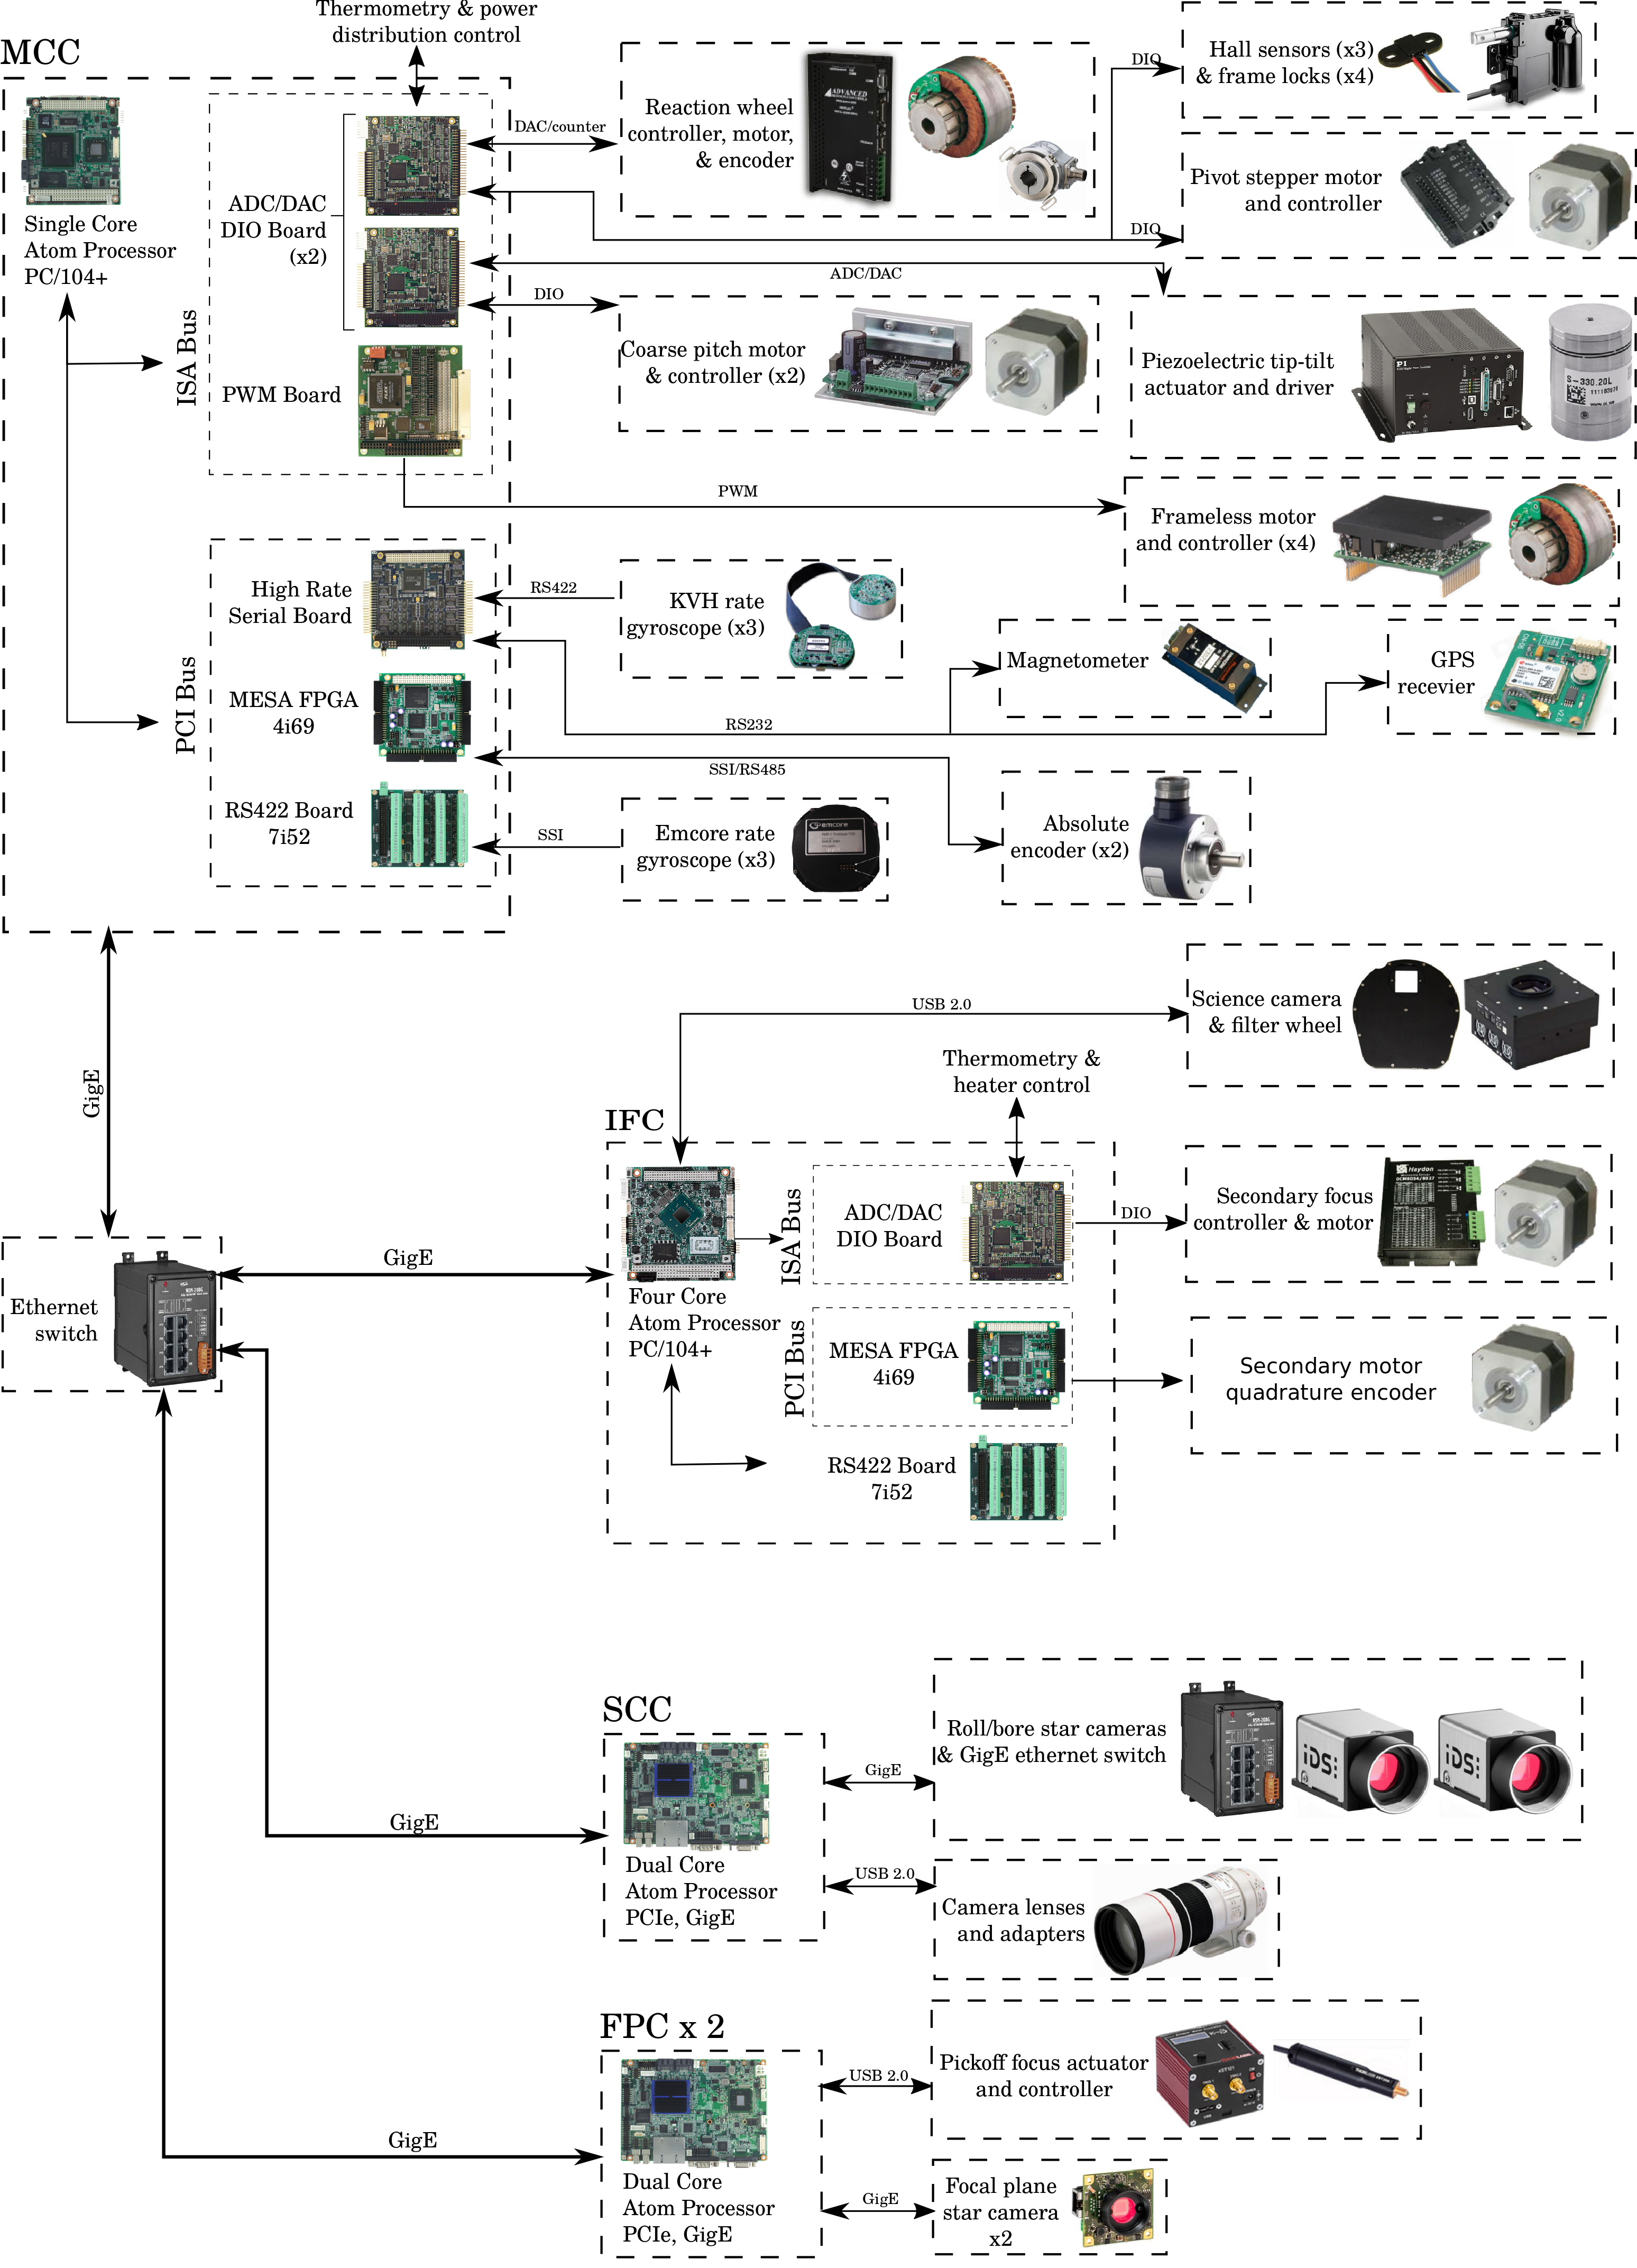
\includegraphics[width=0.95\textwidth]{Hardware/figs/electronics.png}
        \end{center}
        \caption{BIT computer and electronics layout for 2019 flight.}
        \label{fig:electronics}
    \end{small}
\end{figure}

\section{UFO System}
During flight SuperBIT data is nominally transmitted to the ground via satellite communication. Time streams are sent down over each of the
available links (1 MBit LOS, 100 kbps High Gain TDRSS, Iridium) to a central ground computer. Non of the available links are sufficiently fast to transmit SuperBIT's science date during the flight and therefore a hard drive recovery is required.
For a ULDB flight there is a chance that SuperBIT will land in the ocean and thus be unrecoverable. In that scenario the hard drives need to be dropped mid flight separately from the primary payload. The hard drives parachuted down in a raspberry pi controlled compartment known as the UFO system. This system required the design and building of a power control circuit that enables turning on multiple UFOs on and off separately. The design can be seen in \autoref{fig:UFO circuit}. The implementation was soldering 5 copies of the designed circuit in parallel in order to control 3x UFOs and 1x UFO wifi system. The circuit is a simple relay circuit controlled via bit output from the MESA FPGA in the MCC. 

\begin{figure}
    \begin{small}
        \begin{center}
            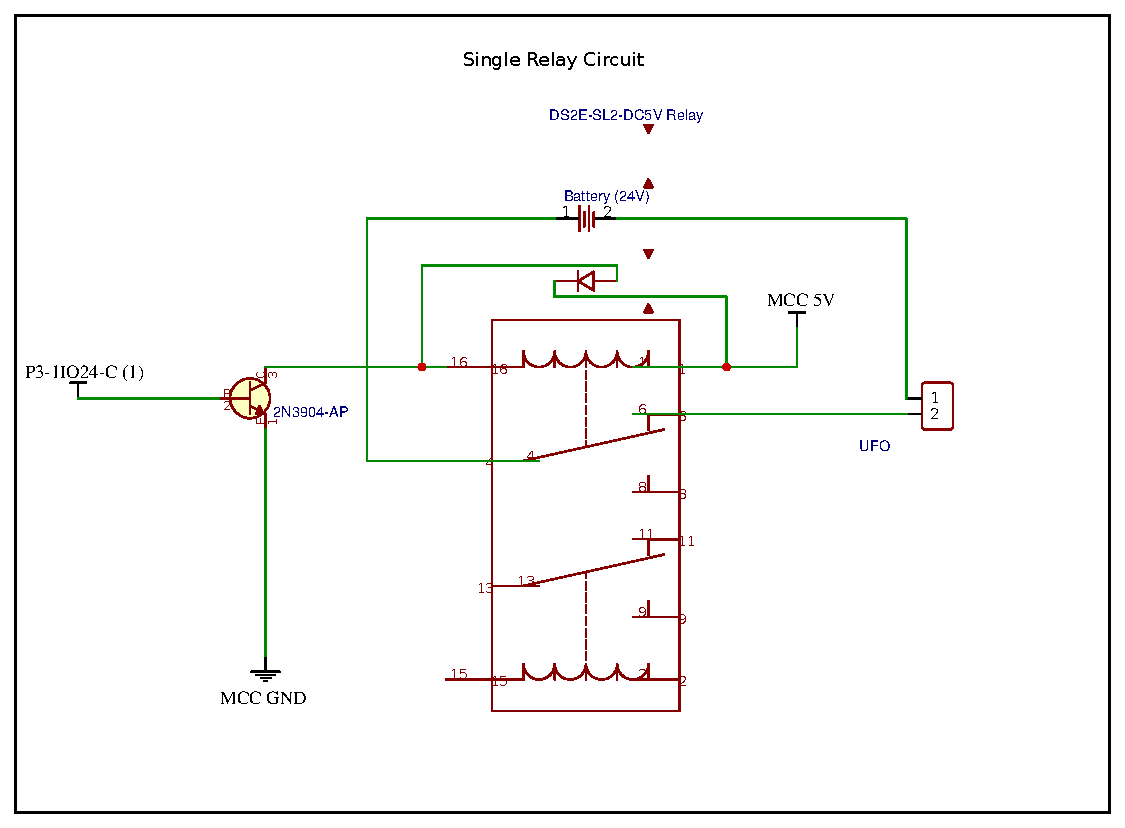
\includegraphics[width=0.95\textwidth]{Hardware/figs/UFO_circ.pdf}
        \end{center}
        \caption{UFO system power control circuit. P3-IO24-C is a sample FPGA output that is fed into a transistor, when the output is pulsed the relay latches on/off turning on the UFO. The UFO is connected directly to SuperBIT's 24V battery system while the relay is isolated and controlled by a 5V power system from the MCC.}
        \label{fig:UFO circuit}
    \end{small}
\end{figure}



\section{Secondary Motors}
characterize them from ajays notes. and from my code work

\section{Baffle Mounting Device}
why do we need it what is mount on it why did it need sorbathane and thermal calcs.

\begin{figure}
    \begin{small}
        \begin{center}
            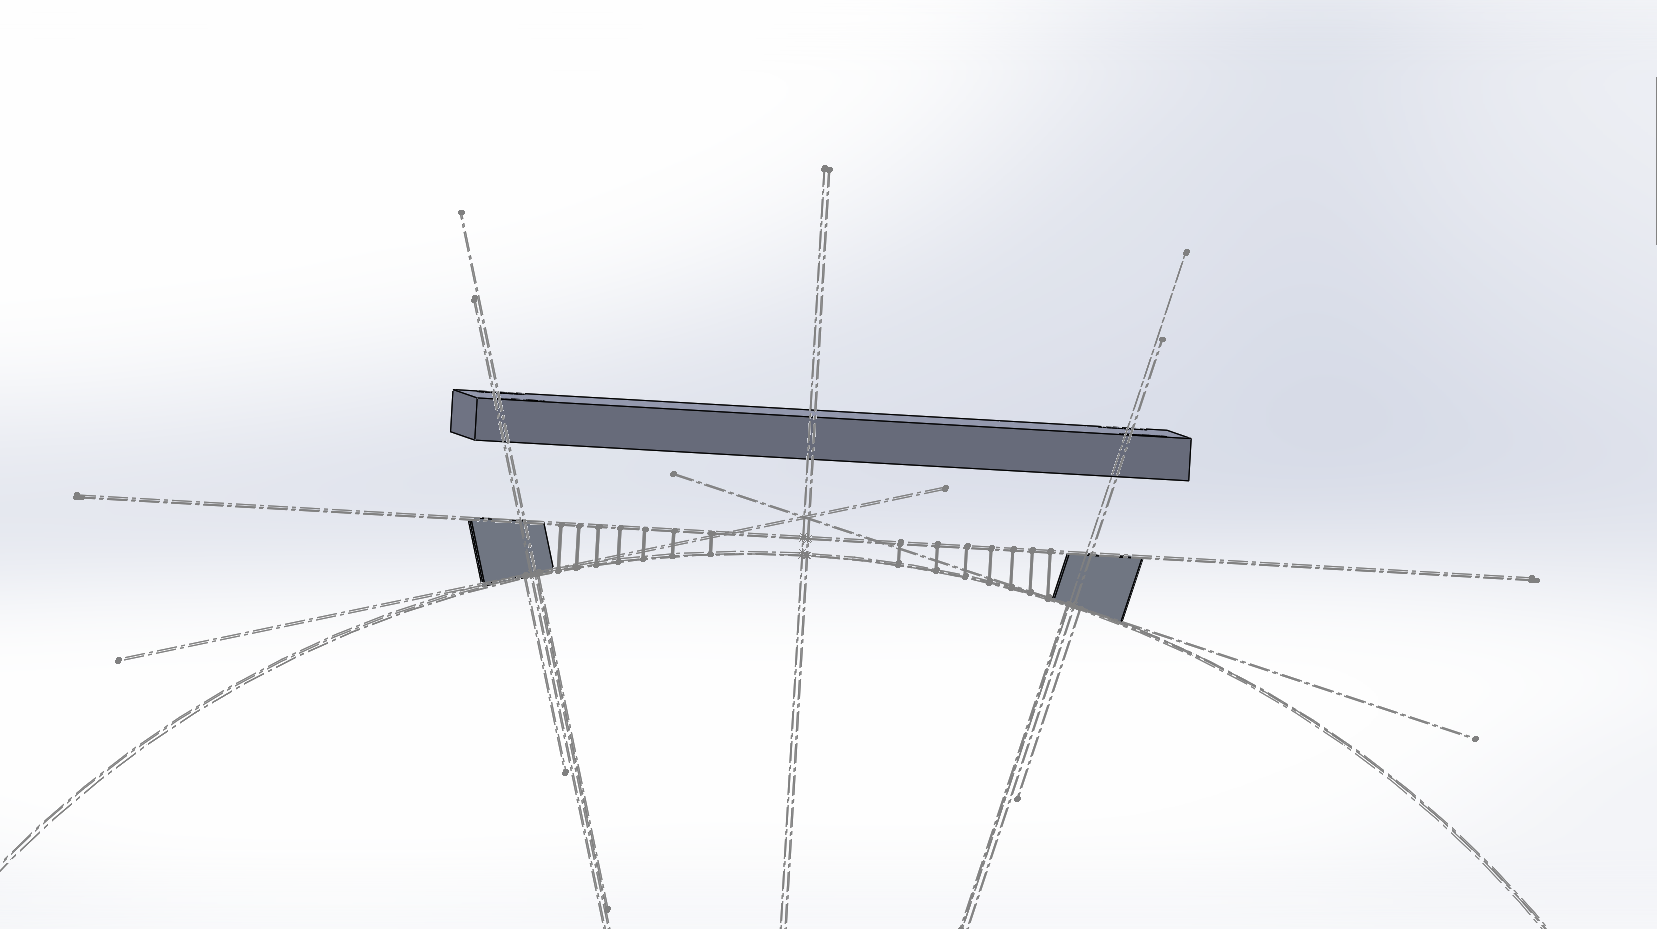
\includegraphics[width=0.95\textwidth]{Hardware/figs/baffle_mount.png}
        \end{center}
        \caption{}
        \label{fig:}
    \end{small}
\end{figure}


\section{Battery Boxes}
why do we need them what do they do and how do they operate.

\begin{figure}
    \begin{small}
        \begin{center}
            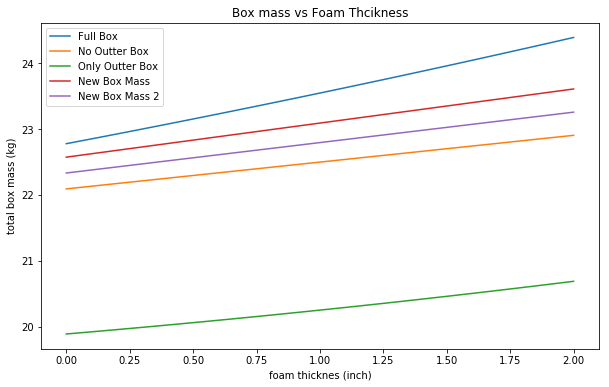
\includegraphics[width=0.95\textwidth]{Hardware/figs/battery_box_mass.png}
        \end{center}
        \caption{}
        \label{fig:}
    \end{small}
\end{figure}

\begin{figure}
    \begin{small}
        \begin{center}
            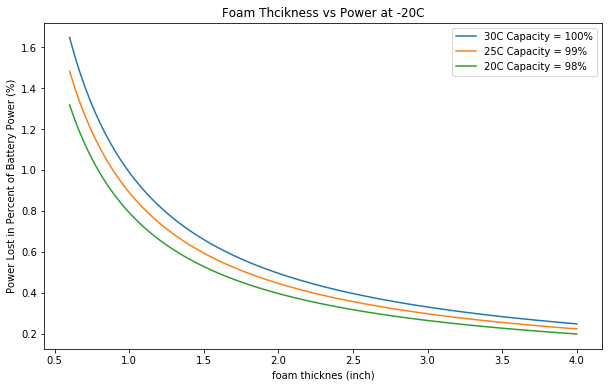
\includegraphics[width=0.95\textwidth]{Hardware/figs/battery_power_loss.png}
        \end{center}
        \caption{}
        \label{fig:}
    \end{small}
\end{figure}


\begin{figure}
    \begin{small}
        \begin{center}
            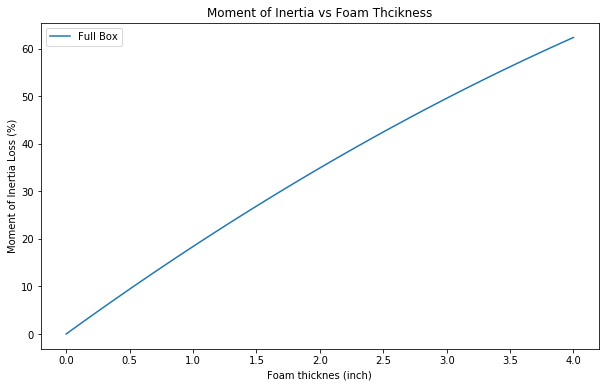
\includegraphics[width=0.95\textwidth]{Hardware/figs/battery_inertia_loss.png}
        \end{center}
        \caption{}
        \label{fig:}
    \end{small}
\end{figure}



\section{Inner Frame Design}


